\documentclass[10pt,a4paper,twocolumn]{jarticle}
%\documentclass[10pt,a4paper]{jarticle}
\usepackage{geometry}
\usepackage{pxchfon}
\usepackage{titlesec}
\usepackage{multicol}
\geometry{left=20mm,right=20mm,top=20mm,bottom=20mm}
\setlength{\columnsep}{10zw}
\usepackage{amssymb,amsmath,amsthm}
\usepackage{amsmath}
\usepackage[dvipdfmx]{graphicx}
\titleformat*{\section}{\normalsize}
\titleformat*{\subsection}{\normalsize}
\titleformat*{\subsubsection}{\normalsize}
\pagestyle{empty}
\renewcommand{\baselinestretch}{1.2}
\usepackage{multirow}

\begin{document}
\twocolumn[
\begin{center}
{\large 卒業論文発表 要旨(2019年度版)\\
ワイヤレス給電システムの最適化のための能率的な動作周波数スイープ\\}
\end{center}
\begin{flushright}
	自動制御研究室\\
	森田 光流 \\
\end{flushright}
\vspace{\baselineskip}
]


\section{緒言}
ワイヤレス給電とはコネクタや金属接点の接触を用いず無線で電力を供給・伝搬することが可能な給電方法である.従来の電気製品の金属接点やコネクタを使用したものは水がかかると水による感電やショートをおこす,配線による転倒などの安全性に関して問題点がある.しかしワイヤレス給電は金属接点がないため前述の問題点を解決することができる.また非金属のものであればコイル間に存在していても送電側と受電側の電力に影響を及ぼさないため,人が立ち寄れない危険な場所や人体の中などにある機器や装置の遠隔操作ができるという点がある
\\ ワイヤレス給電の電力供給の効率の改善には色々と考えられているが本研究においては快適な周波数調整に注目し,最適動作周波数の探索することとした.最適動作周波数は高効率かつ大電力が出力される周波数である.その最適動作周波数探索するためには多くの周波数を測定しなければいけないので測定時間をなるべく短くしたい.しかし,ワイヤレス給電に周波数を送った後安定な電力が出力されるまで時間がかかる.したがって本研究は能率的な周波数スイープを設計し,ワイヤレス給電システムの最適動作周波数を能率的な周波数スイープによる測定・考察を目的とする.
\section{実験}
\subsection{実験回路}
\begin{figure}[h]
	\centering
	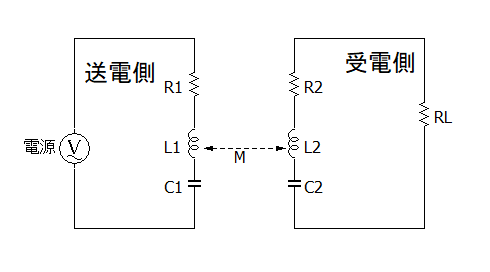
\includegraphics[scale=0.6]{wpt_2020128.png}
	\caption{ワイヤレス給電回路図}
	\label{fig:wpt_kairo}
\end{figure}
ワイヤレス給電は図\ref{fig:wpt_kairo}のように金属接点がない代わりに送電・受電にコイルを用いることにより,送電側の交流電源の電流が時間的に変化することにより受電側の磁束が変化しファラデーの電磁誘導の法則ににより誘導起電力が生じ誘導電流を伝えるという原理である.
なお本研究で使用した実験回路の素子の量は以下の表\ref{tab:para}ようになる.
\begin{table}[h]
	\centering
	\caption{実験回路パラメータ}
	\label{tab:para}
	\begin{tabular}{|l|l|l|}
		\hline
		パラメータ                          & 記号    & 値{[}単位{]}          \\ \hline
		\multirow{2}{*}{コイルの自己インダクタンス} & $L_1$ & $23.6[\mu H]$      \\ \cline{2-3} 
		& $L_1$ & $23.6[\mu H]$      \\ \hline
		相互インダクタンス                      & $M$   & $1.98[\mu H]$      \\ \hline
		\multirow{2}{*}{コイルの内部抵抗}      & $R_1$ & 0.08{[}$\Omega${]}  \\ \cline{2-3} 
		& $R_2$ & 0.08{[}$\Omega${]} \\ \hline
		負荷抵抗                           & $R_L$ & 25{[}$\Omega${]}   \\ \hline
	\end{tabular}
\end{table}
なお,実験回路の共振周波数は以下のとおりである.
\begin{equation}
f_0=99.7kHz \nonumber
\end{equation}

\subsection{周波数スイープ}
実験による最適動作周波数を探索する方法としては周波数スイープが挙げられる.周波数スイープとは一定の時間や速度において7周波数を変化させ出力させる方法である.なお本研究における周波数スイープのやり方でする.
\begin{enumerate}
	\item  一番最初の周波数を回路に送る.なお一番最初の周波数,一番最後の周波数,1つの周波数における測定時間,次の周波数で加算する周波数(以後加算周波数)の量をあらかじめ決めておく必要がある.
	\item 決めた時間で測定する.0.1秒ずつデータが出力される.
	\item 一定時間に達したら,加算周波数を加算し一番最後の周波数に達するまで繰り返す.
\end{enumerate}
 また,先行研究ではワイヤレス給電の周波数スイープをマイコンだけで実行したが,周波数を変更するにあたってわざわざコンパイルしなければならず面倒であった.そこで本研究では周波数スイープの周波数を送る・ワイヤレス給電の電力を受け取る作業をパソコンで自動化するようにした.
\subsection{最適動作判定}
ワイヤレス給電の最適動作周波数であるには前述にも述べたが高電力・高効率であることが重要である.したがって次の計算式(\ref{eq:saiteki})を導入した.なお定数はそれぞれ周波数スイープによって出力された受電側の電力$P_2$と送電側と受電側の出力結果を使って導き出された$効率\eta$である.
\begin{equation}
(最適動作判定)=P_2\eta
\label{eq:saiteki}
\end{equation}
\subsection{能率的な周波数スイープ}
先行研究では,ひとつの周波数を送って次の周波数送るまでの測定時間を10秒だった.しかし,本研究においては多くの周波数による電圧,電流,電力を測りたいがためあまり時間をかけたくない.また加算周波数を低周波数で設定すると確かに正確に測ることが可能だが時間がかかる.逆に大雑把に周波数を取りすぎると正確性に欠ける.したがって周波数スイープが能率的になる周波数の測定時間と,加算周波数の量を事前に決めておく必要がある.表\ref{tab:nouritu}は事前に決めた数値である.
\begin{table}[h]
	\centering

	\caption{測定時間・加速周波数決定値}
	\begin{tabular}{|l|l|}
		\hline
		測定時間  & 1.5s \\ \hline
		加算周波数 & 10k  \\ \hline
	\end{tabular}
\label{tab:nouritu}
\end{table}
\subsection{シミュレーション}
実験をする前に事前にシミュレートしてみた.

\section{実験結果・考察}
\section{今後の方針}

\end{document}
